\documentclass[margin=5pt]{standalone}
\usepackage[utf8]{inputenc}
\usepackage{tikz}
\usepackage{circuitikz}
\usetikzlibrary{circuits.logic.US}
%
\begin{document}
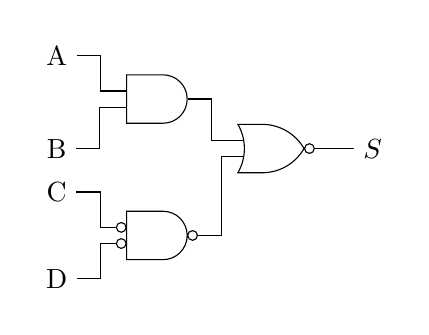
\begin{tikzpicture}[circuit logic US]
    %\node[] at (0,3) { $S = \overline{(A \cdot B) + \overline{(\bar{C} + \bar{D})}} $};
    %
    \matrix[column sep=5mm]{
        \node (iA)  {A}; &                                                   & &\\
                         & \node [and gate, logic gate inputs=nn] (and1) {};  &\\
        \node (iB)  {B}; &                                                   & \node [nor gate] (nor1) {}; & \node (out) {$S$};\\
        \node (iC)  {C}; &                                                   & \\
                         & \node [nand gate, logic gate inputs=ii] (nand1) {}; & \\
        \node (iD)  {D}; &                                                   & \\
    };
    %
    \draw (iA.east) -- ++(right:3mm) |- (and1.input 1);
    \draw (iB.east) -- ++(right:3mm) |- (and1.input 2);
    \draw (iC.east) -- ++(right:3mm) |- (nand1.input 1);
    \draw (iD.east) -- ++(right:3mm) |- (nand1.input 2);
    \draw (and1.output) -- ++(right:3mm) |- (nor1.input 1);
    \draw (nand1.output) -- ++(right:3mm)  |- (nor1.input 2);
    \draw (nor1.output) -- ++(right:3mm) |- (out);
\end{tikzpicture}
\end{document}